\section{Skaner grzbietów książek}
\nextoc

%%%%%%%%%%%%%%%%%

\subsection{Opis działania}
\begin{frame}
    \frametitle{Opis działania z punktu widzenia użytkownika}
    Aplikacja działająca na telefonach z systemem andorid dostaraczająca opis książki, której grzbiet znajduje się na obrazie pochodzącym z kamery.
    
    \begin{center}
    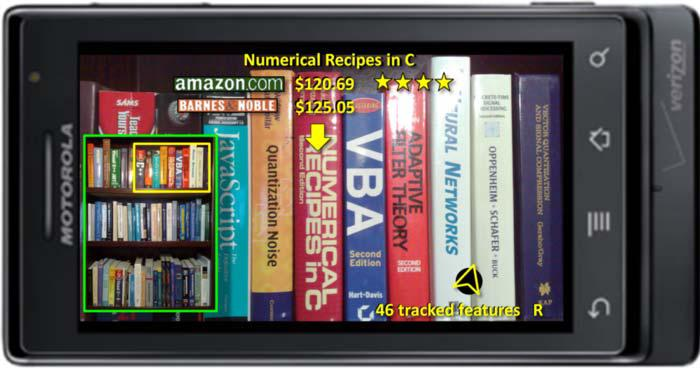
\includegraphics[width=0.6\textwidth]{books_main}
    \end{center}
    
\end{frame}

\subsection{Parametry aplikacji}

\begin{frame}
    \frametitle{Parametry działania aplikacji}
    \begin{itemize}
        \item Rozpoznawanie odbywa się automatycznie, po zatrzymaniu kamery
        \item Czas oczekiwania na wynik rozpoznania: 1s
        \item Lokalizacja książki na pólce z książkami
    \end{itemize}
\end{frame}

%%%%%%%%%%%%%%%%%%%%%%%%

\subsection{Schemat działania}
\begin{frame}
    \frametitle{Schemat działania na telefonie}
    Zadania przeprowadzane na telefonie:
    \begin{itemize}
        \item Analiza ruchu - wykrycie momentu zatrzymania
        \item Wysłanie zarejestrowanego obrazu
        \item Odebranie wyników i wyświetlenie
    \end{itemize}
\end{frame}

\begin{frame}
    \frametitle{Schemat działana na serwerze}
    Na serwerze są przeprowadzane dwie operacje: rozpoznanie książki oraz lokalizacja książki na półce.
    Zadania przeprowadzane przez do rozpoznania książki:
    \begin{itemize}
        \item Segmentacja okładek książek
        \item Rozpoznanie okładki, która znajduje się na środku zdjęcia
    \end{itemize}

    W celu znalezienia książki na półce korzysta się ze zdjęcia przedstawiającego cały regał z książkami.
\end{frame}

\begin{frame}
    \frametitle{Prezentacja działania}
        \url{http://www.youtube.com/watch?v=fWOw2K1TzFk}
\end{frame}
